%卒論中間審査用研究概要テンプレート ver. 1.0

\documentclass[uplatex,twocolumn]{jsarticle}
\usepackage[top=22mm,bottom=22mm,left=20mm,right=20mm]{geometry}
\setlength{\columnsep}{15mm}
\usepackage[T1]{fontenc}
\usepackage{txfonts}
\usepackage{wrapfig}
\usepackage[expert,deluxe]{otf}
\usepackage[dvipdfmx,hiresbb]{graphicx}
\usepackage[dvipdfmx]{hyperref}
\usepackage{pxjahyper}
\usepackage{secdot}

\makeatletter
\renewcommand{\section}{\@startsection{section}{1}{\z@}{0pt}{0.4\Cvs}{\normalfont\raggedright}}
\renewcommand{\subsection}{\@startsection{subsection}{2}{\z@}{\z@}{\z@}{\normalfont}}
\renewcommand{\subsubsection}{\@startsection{subsubsection}{3}{\z@}{\z@}{\z@}{\normalfont}}
\makeatother
%ここから上を編集する必要はない.





%タイトルと学生番号,名前だけ編集すること
\title{\vspace{-5mm}\fontsize{14pt}{0pt}\selectfont クラウドファンディングにおける成功の判別分析}
\author{\normalsize プロジェクトマネジメントコース・ソフトウェア開発管理グループ 矢吹研究室 1242105 三浦泰介}
\date{}
\pagestyle{empty}
\begin{document}
\fontsize{10.5pt}{\baselineskip}\selectfont
\maketitle





%以下が本文
\section{研究の背景}
\makeatletter\renewcommand{\section}{\@startsection{section}{1}{\z@}{0.6\Cvs}{0.4\Cvs}{\normalfont\raggedright}}\makeatother%余白の調整(気にしなくていい)

クラウドファンディング\cite{wiki}と呼ばれる資金調達の手法が世界中で流行りを見せており,その波は日本にも来ている.クラウドファンディングプロジェクトとは必要資金を,インターネットを利用し,不特定多数の支援者から資金提供を募集する資金調達の手法であり,個人規模の小さなプロジェクトでもできるためベンチャー企業や学生から注目を集めている.クラウドファンディングは一般的に資金提供者に対するリターンの形態によって以下の3つに分けることができる.
\begin{enumerate}
 \item 金銭的リターンのない「寄付型」
 \item 金銭的リターンのある「投資型」
 \item 権利や物品を購入することで支援する「購入型」
\end{enumerate}
日本では金融商品取引法が2014年に改正されるまで法規制の問題から,見返りを得ない寄付に近いものか,購入型に限られていたため購入型が主流になっている.日本でプロジェクトを行うことを考え,購入型のプロジェクトの成功率に関わる成功要因を探すこととする.


\section{目的}

クラウドファンディングサイト\cite{makuake}\cite{campfire}\cite{ready}に掲載されているプロジェクトから支援の金額,コースの数など支援者側から見える情報をデータとして集め,決定木を描くことでクラウドファンディングにおける成功要因を明らかにし,クラウドファンディングを用いたプロジェクトを行う際の成功率をあげることを目的とする.

\section{研究方法}

クラウドファンディングサイトを毎日定時に監視し,データを収集を行う.昨年度の結果を元にプロジェクトの内容や代表者から知り得る情報を元に判別分析を行い,成功要因を考察し,成功合否の判別を行う.

\section{成果物のイメージ}

昨年度よりも信憑性の高い決定木を描くこと,まだ見つけていない成功要因を分析結果から考察すること,プロジェクトの成功予測を8割以上で行えるようにすることの三点を成果物の目標とする.
\begin{figure}
\vspace*{-\intextsep}
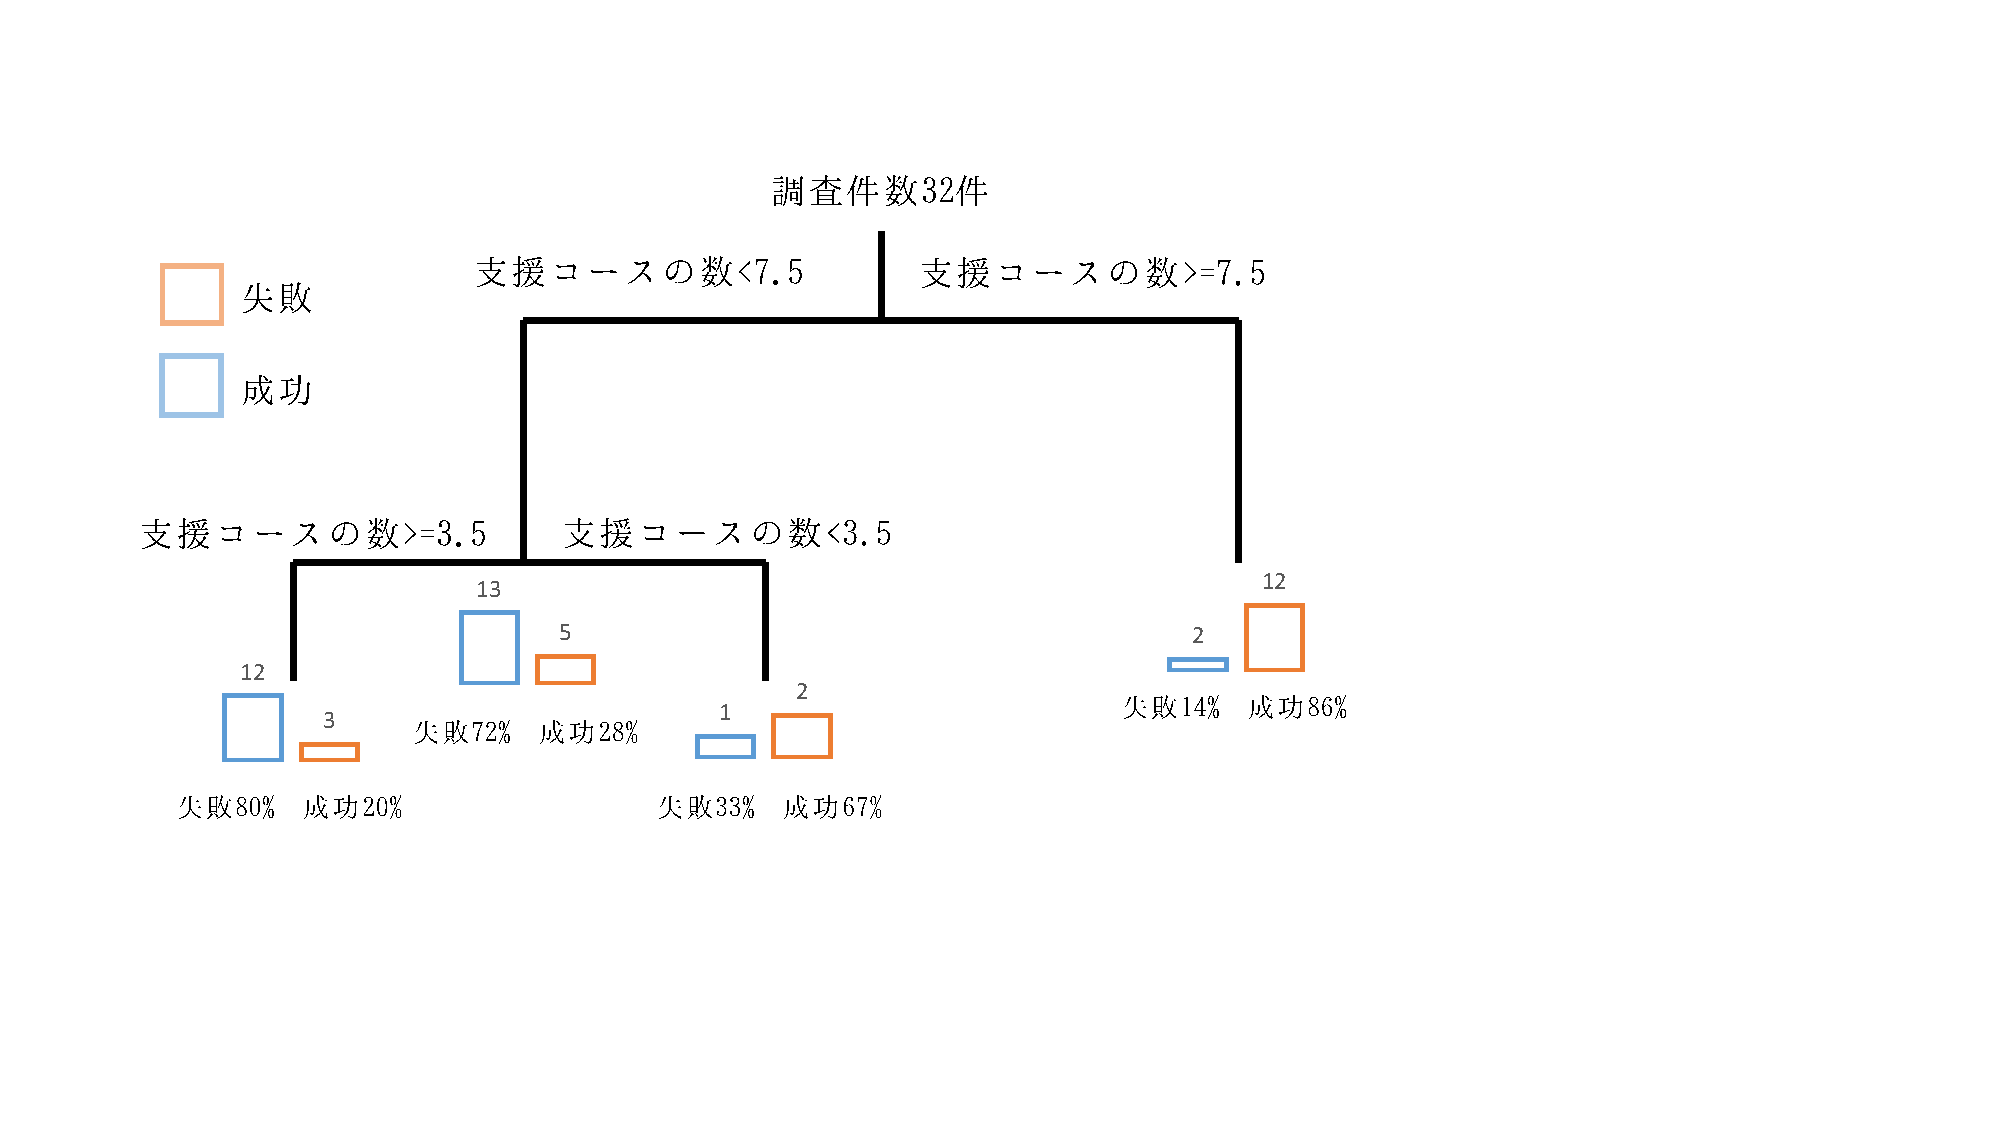
\includegraphics[width=6cm,clip]{figure.pdf}
\caption{昨年度の決定木}\label{サンプル図}
\end{figure}

\section{進捗状況}

一ヶ月分の監視データを集め終え,サイトごとにフォーマットが違うデータを処理する方法を模索している.また随時データを集め続け可能な限り多くのデータを用いて判別分析を行う.

\section{今後の計画}

今までで集めたデータを元にデータ解析を行い,決定木を書くことで成功要因を明らかにする.得られた成功要因から成功予測を行い.終わったプロジェクトの内容を打ち込み,予測と実際の結果の的中率を8割以上にあげることを目標に分析を続ける.





\bibliographystyle{junsrt}
\bibliography{biblio}%「biblio.bib」というファイルが必要.

\end{document}
